%
% Temporal databases
%
A temporal database can generally be seen as a database that manages some temporal aspects in its schema \cite{etzion1998},~\cite{Billiet:Pons:Matthe:DeTre:Pons:2011:BipolarFuzzy}. In subsection \ref{subsec:td-general-concepts}, some main concepts and properties concerning temporal databases and their definitions are presented and explained. In subsections \ref{subsubsec:primary-key} and \ref{subsubsec:consistency}, some main issues of relational temporal databases are presented and discussed. Finally, subsection \ref{Comm-temp} presents an overview of some commercial temporal database systems.

\subsection{\label{subsec:td-general-concepts}Basic Concepts and Properties}
A database schema models some part of reality. As mentioned in the introduction, the part of reality a temporal database schema tries to model, contains some temporal aspects. For example, in this part of reality, some concepts or objects could have time-related or time-variant properties. The modelling of these temporal aspects has to be handled specifically in order for the database to maintain a consistent model of reality.

Thus, a temporal database will contain \emph{temporal values}, i.e. values representing (indications of) time. Temporal values in a temporal database can be classified into the following types based on their interpretation and modelling purpose. The definitions and explanations of these types can be found in \cite{Dyreson1994} and \cite{Nascimento95decisiontime} and more information can be found in \cite{Jensen:1991:IIM:627283.627484}, \cite{Snodgrass:1984:TQL:588011.588041} and \cite{Nascimento95decisiontime}.

\begin{svgraybox}
\vspace{-10pt}
\begin{definition}\textbf{Valid Time}~\cite{Dyreson1994}\\
The \emph{\textbf{valid-time}} (VT) of a fact is the time when the fact is true in the modeled reality.
\end{definition}

\begin{definition}\textbf{Transaction Time}~\cite{Dyreson1994}\\
A database fact is stored in a database at some point in time, and after it is stored, it is current until logically deleted. The \emph{\textbf{transaction-time}} (TT) of a database fact is the time when the fact is current in the database and may be retrieved.
\end{definition}

\begin{definition}\textbf{Decision Time}~\cite{Nascimento95decisiontime}\\
\emph{\textbf{Decision time}} (DT) denotes the time when an event was decided to happen.
\end{definition}

\begin{definition}\textbf{User-defined Time}~\cite{Dyreson1994}\\
\emph{\textbf{User-defined time}} (UDT) is an uninterpreted attribute domain of date and time.
\end{definition}
\vspace{-10pt}
\end{svgraybox}

\emph{Valid times} are usually provided by the user, whereas \emph{transaction-times} are usually system-generated and -supplied \cite{Dyreson1994}. Temporal values of type UDT are not given any extraordinary interpretation and have thus no extraordinary query language support \cite{Dyreson1994}.

A \emph{temporal database} can now formally be defined as follows:

\begin{svgraybox}
\vspace{-10pt}
\begin{definition}\textbf{Temporal Database}~\cite{Dyreson1994}\\
A \emph{\textbf{temporal database}} supports some aspect of time, not counting user-defined time.
\end{definition}
\vspace{-10pt}
\end{svgraybox}

In a relational temporal database, temporal values will of course be in the tuples of the extensions of temporal relations:

\begin{svgraybox}
\vspace{-10pt}
\begin{definition}\textbf{Valid-time Relation}~\cite{Dyreson1994}\\
A \emph{\textbf{valid-time relation}} is a relation with exactly one system supported valid-time.
\end{definition}

\begin{definition}\textbf{Transaction-time Relation}~\cite{Dyreson1994}\\
A \emph{\textbf{transaction-time relation}} is a relation with exactly one system supported transaction-time.
\end{definition}
\vspace{-10pt}
\end{svgraybox}

A \emph{valid-time}, respectively \emph{transaction-time} \emph{relational database} is now defined as containing one or more valid-time, respectively transaction-time relations \cite{Dyreson1994}. Next to this, \emph{bitemporal} relational databases contain both valid-time and transaction-time~\cite{Dyreson1994} and tritemporal databases contain valid-time, transaction-time and decision-time~\cite{Nascimento95decisiontime}.


%Database models can also be classified into \emph{bi-temporal} (both valid and transaction-time) or \emph{tri-temporal}  (bi-temporal and decision-time) models.


A very extensive list of the most well-known temporal database models can be found in ~\cite{Yu1998}. As it is of course necessary to define a consistent way to query the temporal data, there are several proposals concerned with query languages and query language adaptations for temporal databases like ~\cite{TSQL} and ~\cite{Snodgrass98}.




%A \emph{temporal database}~\cite{etzion1998} is a database that manages some aspects of time in its schema~\cite{Dyreson1994}. The reality a temporal database tries to model, contains some temporal notions which have to be handled specifically in order to maintain a consistent modelling behavior. A very extensive list with the most well-known models in temporal databases can be found in ~\cite{Yu1998}. Nevertheless, it is necessary to define some consistent way to query the temporal data. There are several languages for querying temporal databases like TSQL~\cite{TSQL}. In~\cite{Snodgrass98} a proposal to add temporal support to the standard SQL is given.


%\begin{svgraybox}
%The temporal notions in temporal databases can be classified into the following types based on their interpretation and modelling purpose. User-defined time has no interpretation, but the other types do:\\

%	\textbf{Transaction time} \emph{TT}~\cite{Jensen:1991:IIM:627283.627484}: The time when the fact is stored in the database.\\
	
%	\textbf{Valid time} \emph{VT}~\cite{Snodgrass:1984:TQL:588011.588041}: The time when the fact is true in the modelled reality.\\
	
%	\textbf{Decision time} \emph{DT}~\cite{Nascimento95}: The time when an event was decided to happen. \\
%\end{svgraybox}
	


%In the following sections, some of the main points of attention concerning relational temporal databases are explained and discussed.

In the rest of the chapter, the focus will be on concepts and issues concerning valid-time relations and aspects of valid-time relations. For this reason, the next two sections will present and discuss some main issues concerning temporal databases, specifically applied to or presented in the context of valid-time relations.

\subsection{\label{subsubsec:primary-key}Primary Keys in Valid-time Relation Design}
Generally, when designing a relation based on a relational database model, a subset of the relation's attribute set is usually chosen as primary key. The values of a tuple for these attributes will then uniquely determine this tuple, hence no two distinct tuples may have the exact same values for every attribute in this primary key. Next to attributes unrelated to time, a valid-time relation schema will typically contain one or more attributes which model the valid-time aspects and behavior of the real objects and concepts modelled by the relation schema. In this work, these attributes are called \emph{valid-time attributes}. In valid-time relation extensions, distinct tuples can exist containing the exact same values for every attribute except the valid-time attributes. These distinct tuples represent distinct versions of the same real object or concept, valid during different time periods. To allow the existence of such tuples when designing a valid-time relation using a relational database model, the most common solution is to include the valid-time attributes in the primary key.
%One of the first tasks in the design of a database is the choice for the primary key. In a temporal database, the most common solution for the choice of the primary key is to extend the primary key with the temporal value. Nevertheless, when dealing with uncertainty in the temporal values, the solution is usually to create a version identifier otherwise the primary key have uncertainty which should be avoided.

The following example illustrates this primary key issue.

\begin{example}
\label{ex:pk}
Consider the example valid-time relation visualized in table \ref{table:example-database}, which models when certain people worked as employees in a certain company and under whose supervision they worked during that time. The valid-time attributes `Start' and `End' describe the year when an employee started, respectively finished working for the company. For example, the last tuple visualized in table \ref{table:example-database} represents that the employee represented by this tuple started working for the company in 2005 and finished in 2009. The attributes `Name', `Birthday' and `Supervisor' describe respectively the name, birthday date and unique identifier of the supervisor of an employee in the time during which he or she worked for the company. When correct, the date of an employee's birthday never changes and as such, the modelling of birthday dates has no effect on the database consistency. The `Birthday' attribute thus describes UDT values. The attribute `ID' describes employee identifiers. For each tuple, this identifier (a number) uniquely identifies the employee represented by the tuple. 

Now consider $\{$ID$\}$ being the primary key and consider the company wanting to hire Sarah again in 2010. This would be represented by another tuple in the relation, containing value 4 for attribute `ID'. The existence of such a tuple is of course not allowed by the primary key, because it would mean the existence of two distinct tuples containing value 4 for attribute `ID'. This problem can now be solved by defining a new primary key: $\{$ID, Start, End$\}$, which allows for the existence of distinct tuples with value 4 for attribute `ID', as long as they have different values for attributes `Start' or `End'. The resulting relation is shown in table~\ref{table:example-database-with-new-pk}.
%Consider the example database visualized in table \ref{table:example-database}. It contains data representing employees in a company, and two temporal values which represent a valid-time interval. Consider now that we want to hire Sarah again. That is not possible because of the primary key (ID) does not allow to insert again the row Sarah but with a different start and end time. In some models this is resolved by adding to the primary key both values Start and End years. The resulting database allows to insert a new row where Sarah the year 2010. But this modification also allows to insert spurious values e.g., inconsistent time periods (see last row in table \ref{table:example-database-with-new-pk}).

\end{example}
%\begin{note}
%The attribute `Age' in the presented relations visualized in tables~\ref{table:example-database},~\ref{table:example-database-with-new-pk} and~\ref{table:example-database-update} describes the age of an employee and is included as an example of . In reality, the birthday of the employee should be stored in the database, rather than the age, because the age 
%In the presented relations visualized in tables~\ref{table:example-database},~\ref{table:example-database-with-new-pk} and~\ref{table:example-database-update}, the value of a tuple for attribute `Supervisor' should actually contain the unique identifier of the supervisor of the employee represented by the tuple. the relation `Supervisor' stores the ID of the employee. To improve the readability of the example, the tables show the name of the employee. Note also that the field for the age is expressed as the age in years whereas the value stored in the database is the birthday.
%\end{note}



%Extending a primary key to include temporal attributes allows for the insertion of spurious values, for example representing temporal inconsistencies. This is shown in table \ref{table:example-database-with-new-pk}, where it seems Sarah was rehired in 2007 and fired in 2008.

%\vspace{-10pt}

\begin{table}
\centering
\caption{Example relation modelling the employees of a company. Values for the `Birthday' attribute are visualized here in `dd/mm/yyyy' format.}
\begin{tabular}{c c c c c c }
\hline
\textbf{ID} & \textbf{Name} & \textbf{Birthday} & \textbf{Supervisor} & \textbf{Start} & \textbf{End} \\ \hline
1 & Peter & 24/10/1985 & 3 &  2010 & - \\
2 & Maria & 03/04/1984 & 3 & 2001 & - \\
3 & John & 21/02/1964 & - &  1999 & - \\
4 & Sarah & 29/11/1985 & 2 &  2005 & 2009 \\
\hline 
\end{tabular}
\label{table:example-database}

%\vspace{10pt}


\end{table}

%\vspace{-25pt}


%\vspace{-10pt}

\begin{table}
\centering
\caption{Example relation after including the valid-time attributes in the primary key and adding a tuple.}
\begin{tabular}{c c c c c c }
\hline
\textbf{ID} & \textbf{Name} & \textbf{Birthday} & \textbf{Supervisor} & \textbf{Start} & \textbf{End} \\ \hline
1 & Peter & 24/10/1985 & 3 &  2010 & - \\
2 & Maria & 03/04/1984 & 3 & 2001 & - \\
3 & John & 21/02/1964 & - &  1999 & - \\
4 & Sarah & 29/11/1985 & 2 &  2005 & 2009 \\
4 & Sarah & 29/11/1985 & 2 &  2010 & - \\
%4 & Sarah & 29/11/1985 & 2 &  2007 & 2008 \\
\hline 
\end{tabular}
\label{table:example-database-with-new-pk}
\end{table}

%The next subsection is concerned with another interresting issue.

\subsection{\label{subsubsec:consistency}Consistency in Valid-time Relation Content Modification}
The solution presented in subsection~\ref{subsubsec:primary-key} concerns relation design and consists of including the valid-time attributes in the primary key. Unfortunately, implementing this solution as such allows for the existence of records whose values imply inconsistencies with respect to the modelling of reality.

Consider a valid-time relation of which the primary key can be partitioned into two sets of attributes. One set contains attributes totally unrelated to time, for which the values of a record allow to uniquely identify the object or concept represented by the record. The other set contains the valid-time attribute(s). Because the valid-time attribute(s) is(are) included in the primary key, the existence of distinct records with exactly the same values for all time-unrelated attributes and distinct values for at least one valid-time attribute is not prohibited. Thus, inserting such records into the relation is not prohibited either, even if the information represented by the values for the valid-time attributes shows clear inconsistencies. An example.

\begin{example}
\label{ex:prob}
Consider the example valid-time relation visualized in table \ref{table:erconsistency}, which is based on the relation visualized in table~\ref{table:example-database}. The primary key is again $\{$ID, Start, End$\}$. The last record in the relation represents a person named `Sarah' started working for the company in 2007 and finished in 2008, with supervisor `John'. However, the fourth record represents the same person (the value for attribute `ID' is the same) started working for the company in 2005 and finished in 2009, with supervisor `Maria'. The intention is clear: Sarah worked in the company from 2005 to 2009, first for Maria, then for John, then again for Maria. It is of course possible for an employee to change supervisors, but it is of course impossible for a person to start working in the same company twice at different times, for different supervisors, without stopping to work for one in between, as it is impossible to stop working for a supervisor twice at different times, without working for another one in between. The valid-time information represented by the last record is clearly not consistent with the valid-time information represented by the fourth record, or vice versa.
\end{example}

\begin{table}
\centering
\caption{Example relation with records whose values for the valid-time attributes violate consistency.}
\begin{tabular}{c c c c c c }
\hline
\textbf{ID} & \textbf{Name} & \textbf{Birthday} & \textbf{Supervisor} & \textbf{Start} & \textbf{End} \\ \hline
1 & Peter & 24/10/1985 & 3 &  2010 & - \\
2 & Maria & 03/04/1984 & 3 & 2001 & - \\
3 & John & 21/02/1964 & - &  1999 & - \\
4 & Sarah & 29/11/1985 & 2 &  2005 & 2009 \\
%4 & Sarah & 29/11/1985 & 2 &  2010 & - \\
4 & Sarah & 29/11/1985 & 3 &  2007 & 2008 \\
\hline 
\end{tabular}
\label{table:erconsistency}
\end{table}

The most usual approach to deal with this inconsistency problem is to adapt the DML used by the DBMS, as to enforce consistency towards time with respect to the modelled reality.

\begin{example}
Consider the problem presented in example~\ref{ex:prob}. The inconsistency arises when the last record in table~\ref{table:erconsistency} is inserted. Because the record's values for the valid-time attributes differ from those of the fourth record, the last record is accepted. The DML statement used was (the table is called `Employees'):

\begin{verbatim}
INSERT INTO Employees VALUES
 (4, `Sarah', `29/11/1985', 3, 2007, 2008);
\end{verbatim}

\noindent
The inconsistency problem can now be solved by replacing this statement with:

\begin{verbatim}
UPDATE Employees SET `End' = `2007' WHERE
 (ID = 4) AND (Start = 2005) AND (End = 2009);
INSERT INTO Employees VALUES
 (4, `Sarah', `29/11/1985', 3, 2007, 2008);
INSERT INTO Employees VALUES
 (4, `Sarah', `29/11/1985', 2, 2008, 2009);
\end{verbatim}

\noindent
The resulting relation is visualized in table~\ref{table:example-database-update}.

\end{example}

%As stated in subsection \ref{subsubsec:primary-key}, one of the main issues concerns the insertion of spurious values in a relation. Another issue concerns the possible breach of consistency when updating records. The most usual approach to deal with this is to change the database DML to enforce the consistency with which the temporal relation models the temporal properties of the part of reality the relation models. An example of such DML adaptation is given below.

%The consistence mechanism in a temporal database is usually re-defined. The main problem is the insertion of spurious values in the database, as shown in example \ref{ex:pk}, in table \ref{table:example-database-with-new-pk}. The most usual solution is to re-define the DML (\emph{Data Manipulation Language}). e.g., the \emph{update} sentence is redefined as two sentences an update and a create sentence as illustrated in the following example.

%\begin{example}
%Consider the database in table \ref{table:example-database}. The employee with ID=3 (John) works now for the employee with ID= 4 (Sarah). The update is made in the following sentence:

%The following \emph{update} sentence:

%\begin{verbatim}
%Update Employees set 'Works for' = 4 where ID=3;
%\end{verbatim}

%Is translated into the following two sentences: an update for the last version of the row and an insert sentence for the new version. Consider that the time in the  system is the year 2010. Then, the update sentence showed above is translated into:

%\begin{verbatim}
%Update Employees set EndYear = 2010 where ID=3;
%Insert into Employees values (3,John,52,Sarah,2010,-);
%\end{verbatim}

\begin{table}
\centering
\caption{Example relation updated maintaining consistency.}
\begin{tabular}{c c c c c c }
\hline
\textbf{ID} & \textbf{Name} & \textbf{Birthday} & \textbf{Supervisor} & \textbf{Start} & \textbf{End} \\ \hline
1 & Peter & 24/10/1985 & 3 &  2010 & - \\
2 & Maria & 03/04/1984 & - & 2001 & - \\
3 & John & 21/02/1964 & - &  1999 & 2010 \\
3 & John & 21/02/1964 & - &  2010 & - \\
4 & Sarah & 29/11/1985 & 2 &  2005 & 2007 \\
4 & Sarah & 29/11/1985 & 3 &  2007 & 2008 \\
4 & Sarah & 29/11/1985 & 2 &  2008 & 2009 \\
\hline 
\end{tabular}
\label{table:example-database-update}

%\vspace{10pt}


\end{table}

%\vspace{-25pt}

%Table \ref{table:example-database-update} shows the resulting database after the update sentence.

%\end{example}


\subsection{\label{Comm-temp}Commercial Temporal Database Systems}
Several commercial temporal DBMS exist. Table \ref{table:commercial-temporal-db} gives an overview of some of the more well-known temporal DBMS and provides references for more information. 

Oracle workspace manager~\cite{oracle2009} and TimeDB~\cite{timedb2005} are libraries for dealing with time in OracleDB. On another note, TimeDB and Postgree Temporal~\cite{posgree2009} are similar: both are simple implementations that implement a subset of the Allen operators and some operations for the creation and manipulation of temporal attributes (valid-time, transaction-time or both times are supported). Teradata~\cite{teradata2011} is mainly a business intelligence system designed for data mining. Secondo~\cite{Dieker2000} is an extensible database system in which the core of the database may be replaced by a customized algebra. It is designed for non-standard applications and it supports both valid and transaction-times. 

 The most complete implementation is Workspace Manager.

Unfortunately, none of these systems take data imperfections into account, neither in data storage nor in querying.

\begin{table}
\centering
\caption{Commercial Temporal Database Systems. }
\begin{tabular}{c c c c c c }
\hline
\textbf{Name} & \textbf{Time Supported} & \textbf{Comments} & \textbf{Reference}  \\ \hline
Oracle Workspace Manager & VT and TT. & Package for Oracle DB. & \cite{oracle2009}\\
TimeDB & VT and TT. & Interface for Oracle DB. & \cite{timedb2005}\\
Postgree Temporal & VT. & Package for Postgree SQL. & \cite{posgree2009}\\
Teradata & VT and TT. & Used for data-mining. & \cite{teradata2011}\\
Secondo & VT and TT. & Spatio-temporal database. & \cite{Guting} \\
\hline 
\end{tabular}
\label{table:commercial-temporal-db}

%\vspace{10pt}


\end{table}

%\subsubsection{Oracle Workspace Manager}
%
%\begin{figure}
%\centering
%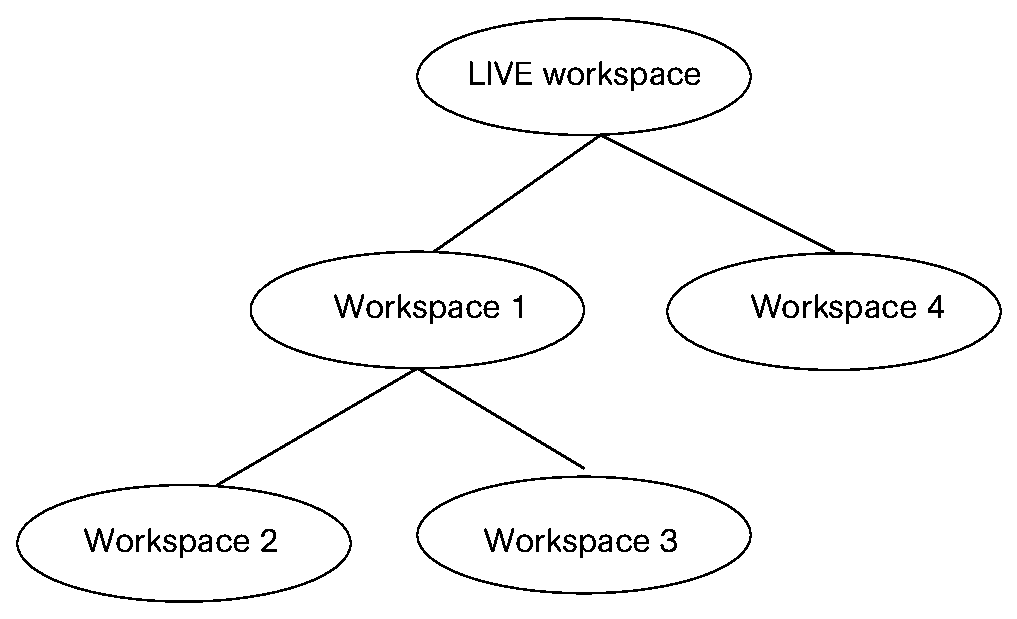
\includegraphics[scale=0.5]{graphs/workspaceTopology.eps}
%\caption{A sample topology in the workspace manager.}
%\label{fig:workspace-topology}
%\end{figure}
%
%Oracle workspace manager \cite{OraE118602} package allows to get several versions of the data in the same database. It is also possible to version only a table. The main benefits of this are two:
%
%\begin{itemize}
%\item
%Organization and optimization of data in a hierarchical frames: It is possible to create a frame of time (a workspace) and work only with that partial version of the data. It is provided a mechanism to merge data among different workspaces and to solve conflicts. The organization of data in these workspaces for very large tables result in smaller time access.
%\item
%Valid time as well as transaction-time are managed by the system. Each update sentence makes a change in the versioning of a row.
%\end{itemize}
%
%When a table is versioned, the system creates a few tables and views as well as auxiliary structures to allow keep several version of the data, while keeping the primary key defined by the user.
%
%A workspace is a logical group of a set of changes (versions of tuples) and allows consistent access, thus the user always obtain the correct data version. Workspaces are ordered in a hierarchy. The top level is called LIVE workspace (see figure \ref{fig:workspace-topology}).  \\
%
%The system only makes a copy of a tuple if it is changed. In order to access different versions of the tuple, the context must be changed. Also, it is not necessarily to modify the SQL code to access to versioned tables.\\
%%When a table is versioned, it is renamed as table\_LT. Here is stored all the data for the information together metadata for the versioning. An auxiliary table is created with the workspace metadata with the name table\_AUX. A view is created with the name of the original table to allow querying without versioning.

